\chapter{I Interviewed 30 Billionaires: What the Arithmetic Reveals}

This lecture from School of Hard Knocks, curated by LazyingArt LLC, opens by turning the camera back on its usual operator. The interviewer, who ordinarily extracts rules from billionaires, athletes, and celebrities, is now asked to answer for his own scale, his own method, and his own income. That reversal matters. It gives the lecture an immediate quantitative backbone. From there the talk unfolds as a ranked countdown, and each rank follows the same rhythm: a clip, a compression, and then a harder doctrine. The mathematics here is not textbook finance. It is the arithmetic of stacked revenue, compounding horizons, retained capital, marketing reach, competition density, and finite remaining life.

\begin{remark}
No validated mathematical screenshots survive for this lecture. Every figure below is therefore a cautious reconstruction from the transcript, meant to clarify the spoken logic rather than to replace visual evidence that does not exist.
\end{remark}

\section{Opening inversion and the host's own business arithmetic}

The lecture begins with a montage of names and faces. Shaquille O'Neal, Tom Brady, Tom Cruise, Mark Cuban, Michael Rubin, and the richest men in Dubai appear in rapid succession. The point is not decoration. The montage establishes that the host has stood near unusual concentrations of wealth and influence. Only after that authority is in place does the guest flip the script: instead of the host asking rich people how they got rich, the host must answer the question himself.

The first response is numerical. The lecture does not wait for abstractions:
\begin{align}
N_{\mathrm{B}} &> 30, &
N_{\mathrm{I}} &> 1000, \\
R_m &> \$700{,}000, &
R_y &> \$6{,}000{,}000.
\end{align}
Here \(N_{\mathrm{B}}\) denotes the number of billionaires interviewed in roughly four years, \(N_{\mathrm{I}}\) the total number of interviews, \(R_m\) recent monthly business revenue, and \(R_y\) projected yearly business revenue.

That is the first real spine of the lecture. The host is no longer only curator; he becomes a worked example. The guest then asks the natural follow-up: how can an interview brand generate that kind of revenue? The answer is not a single line item. The host says that he has built businesses around the channel: a marketing agency, a consulting company, brand partnerships, ad revenue, and a subscription community. A cautious reconstruction is
\begin{equation}
R = R_{\mathrm{agency}} + R_{\mathrm{consult}} + R_{\mathrm{brand}} + R_{\mathrm{ads}} + R_{\mathrm{sub}},
\end{equation}
with \(R_{\mathrm{sub}}\) standing for the subscription or community stream.

The lecture is already telling us something durable. Wealth at scale is not described as a paycheck. It is described as layered extraction around a core engine of attention.

\begin{figure}[h]
\centering
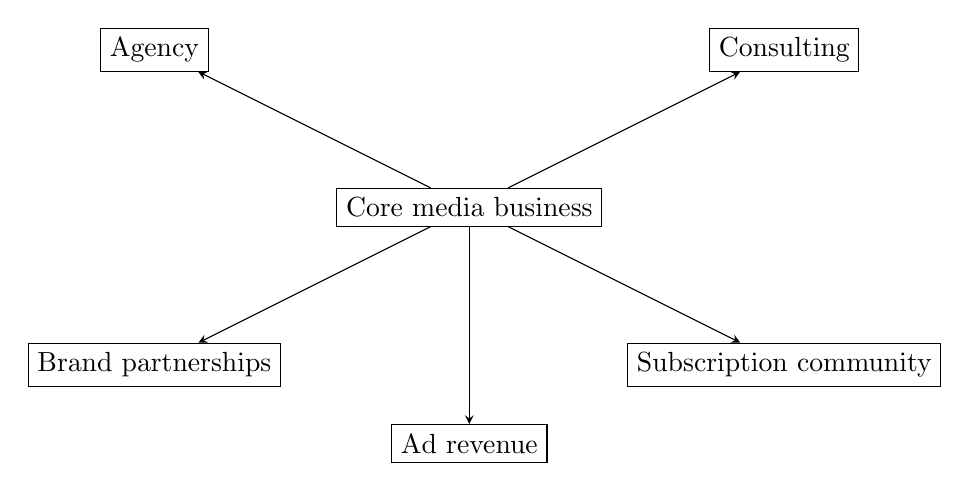
\begin{tikzpicture}[>=stealth]
\node[draw, rectangle] (core) at (0,0) {Core media business};
\node[draw, rectangle] (agency) at (-4,2) {Agency};
\node[draw, rectangle] (consult) at (4,2) {Consulting};
\node[draw, rectangle] (brand) at (-4,-2) {Brand partnerships};
\node[draw, rectangle] (ads) at (0,-3) {Ad revenue};
\node[draw, rectangle] (sub) at (4,-2) {Subscription community};

\draw[->] (core) -- (agency);
\draw[->] (core) -- (consult);
\draw[->] (core) -- (brand);
\draw[->] (core) -- (ads);
\draw[->] (core) -- (sub);
\end{tikzpicture}
\end{figure}

Only after this self-accounting does the guest issue the lecture's formal challenge: from well over a thousand interviews, give us the fifteen greatest pieces of advice. The chapter must keep that challenge in view, because the rest of the lecture proceeds not as continuous exposition but as a ladder of ranked compressions.

\section{Advice, credibility, and the right to be heard}

At number \(15\) the lecture does not yet tell us how to scale a business. It first tells us how to filter counsel. Will Smith gives the line that sets the tone: taking advice from someone who has not done what you want to do is nearly insane. The host restates it more sharply: never take advice from someone you would not trade places with.

We may formalize the filter without pretending that the lecture is giving a theorem:
\begin{definition}
A piece of advice is operationally admissible only if the speaker has already done the thing being recommended.
\end{definition}

In symbols,
\begin{equation}
\mathrm{admissible}(x) \Rightarrow x \text{ has already done the target thing.}
\end{equation}

This is a modest equation, but it performs real work. The lecture is clearing noise out of the channel before it starts discussing money, investing, or scale.

At number \(14\), Robert Herjavec pushes the same clearing operation into the domain of access. The middle of this clip is badly garbled in the transcript, so we should keep only the stable line. The lecture rejects the lazy slogan that success depends mainly on already knowing the right people. Herjavec begins without money or family-business entry. The host's takeaway is the usable part: one must build visible wins, earn credibility, and only then expect high-level people to take the call.

The cleanest reconstruction is
\begin{equation}
\text{wins} \longrightarrow \text{credibility} \longrightarrow \text{access}.
\end{equation}

\begin{figure}[h]
\centering
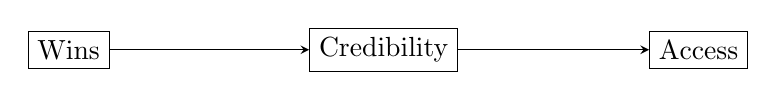
\begin{tikzpicture}[>=stealth]
\node[draw, rectangle] (wins) at (0,0) {Wins};
\node[draw, rectangle] (cred) at (4,0) {Credibility};
\node[draw, rectangle] (access) at (8,0) {Access};

\draw[->] (wins) -- (cred);
\draw[->] (cred) -- (access);
\end{tikzpicture}
\end{figure}

We should notice the order. The lecture first tells us whom to hear, then tells us how one becomes worth hearing. That is why these lessons come before the financial mechanics. The speaker is building the right to make claims.

\section{Investing, retention, and the anti-consumption rule}

At number \(13\), Ashley Fox shifts the lecture from epistemic hygiene to capital. Her line is simple and severe: wealthy people put their money to work. They do not merely leave it in a savings account. The host immediately says that after interviewing thirty billionaires, this is the golden rule.

\subsection{Question \& Answer}

Can one save one's way to wealth? In the logic of this lecture, no. Mere saving adds only the next contribution. Investing adds both the contribution and the return on the existing stock:
\begin{align}
W_{t+1}^{\mathrm{saved}} &= W_t + s_t, \\
W_{t+1}^{\mathrm{invested}} &= (1+r_t)W_t + s_t.
\end{align}
Here \(W_t\) is wealth at time \(t\), \(s_t\) is fresh saving, and \(r_t\) is the return on deployed capital. The lecture is not teaching portfolio theory. It is drawing a sharp line between additive accumulation and multiplicative accumulation. That is enough.

The long interlude on ``generational wealth day'' follows immediately after this point, and we should not erase it completely. In final prose it should be brief, but its structural role matters. The host monetizes access to investment expertise at precisely the moment when the lecture has established that investment knowledge is scarce and consequential. The interruption is therefore not random. It is itself an example of how the speaker turns access and network into product.

At number \(12\), the lecture returns to the countdown with a Houston multimillionaire. The scale anchor is strong:
\begin{equation}
Y_{\mathrm{Houston},2020} \approx \$16{,}000{,}000.
\end{equation}
But the lesson is not luxury. It is delayed luxury. The speaker says he was making roughly \(\$30{,}000\) a month with only about \(\$3{,}000\) to \(\$4{,}000\) in overhead, and that the visible lifestyle upgrade came only after millions had already been saved. The line that remains is the one the host repeats several times: stay small enough, long enough, and you will be big enough soon enough.

The host then makes the rule personal. He says that when he and his partners were making about \(\$30{,}000\) a month in profit, they were paying themselves only about \(\$2{,}000\). The transcript is unclear about whether this draw is per partner or total, and that ambiguity must stay visible. Even so, the direction of the arithmetic is plain. Low extraction preserves internal capital.

A general update rule is
\begin{equation}
K_{t+1} = K_t + \Pi_t - D_t + I_t,
\end{equation}
where \(K_t\) is retained business capital, \(\Pi_t\) is profit, \(D_t\) is owner draw, and \(I_t\) is explicit reinvestment back into growth.

If we momentarily suppress the bookkeeping distinction between retained profit and reinvestment, the host's anecdote becomes a worked example:
\begin{align}
\Delta K_m &= \Pi_m - D_m \\
&\approx \$30{,}000 - \$2{,}000 \\
&\approx \$28{,}000.
\end{align}
That is the lecture's anti-consumption arithmetic. It is not asceticism for its own sake. It is a resilience strategy. Low draw gives the business a cushion in weak months and ammunition in strong ones.

\begin{figure}[h]
\centering
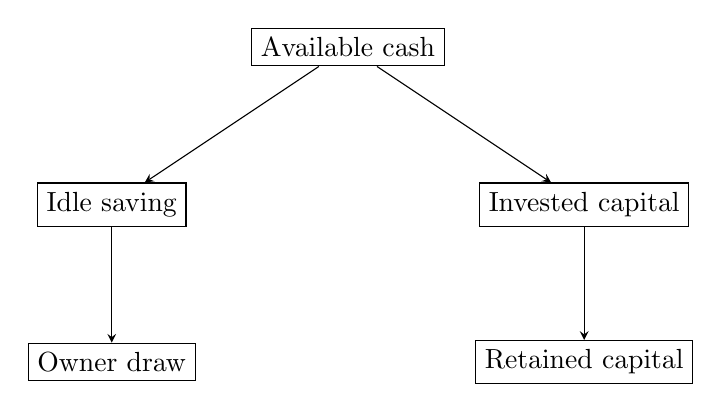
\begin{tikzpicture}[>=stealth]
\node[draw, rectangle] (cash) at (0,2) {Available cash};
\node[draw, rectangle] (save) at (-3,0) {Idle saving};
\node[draw, rectangle] (invest) at (3,0) {Invested capital};
\node[draw, rectangle] (draw) at (-3,-2) {Owner draw};
\node[draw, rectangle] (retain) at (3,-2) {Retained capital};

\draw[->] (cash) -- (save);
\draw[->] (cash) -- (invest);
\draw[->] (invest) -- (retain);
\draw[->] (save) -- (draw);
\end{tikzpicture}
\end{figure}

\section{Long horizons and omnipresence}

At number \(11\), Reid Hoffman shifts the lecture from short-run retention to long-run horizon. He is asked a deliberately compressed question: if one had to make a billion dollars in one year, what would one do? His answer is not to solve the one-year problem inside its own frame. It is to reject the frame entirely. He says he almost never plays a one-year game. He plays a ten-year game.

The clip is anchored by the scale of the man answering. LinkedIn was sold to Microsoft for
\begin{equation}
V_{\mathrm{LinkedIn}} = \$26{,}000{,}000{,}000.
\end{equation}
The host then generalizes immediately: billionaires think in decades, not days.

We can write the horizon change first in its bare form,
\begin{equation}
T_{\mathrm{short}} = 1 \text{ year}, \qquad T_{\mathrm{long}} = 10 \text{ years},
\end{equation}
but the lecture is really pointing us toward the mechanism that only appears on the longer interval:
\begin{equation}
V_T = V_0 \prod_{t=1}^{T} (1+g_t).
\end{equation}
This is a cautious standard reconstruction, not a formula spoken verbatim. It is the cleanest mathematical statement of what the lecture means by compounding to ten years.

\begin{figure}[h]
\centering
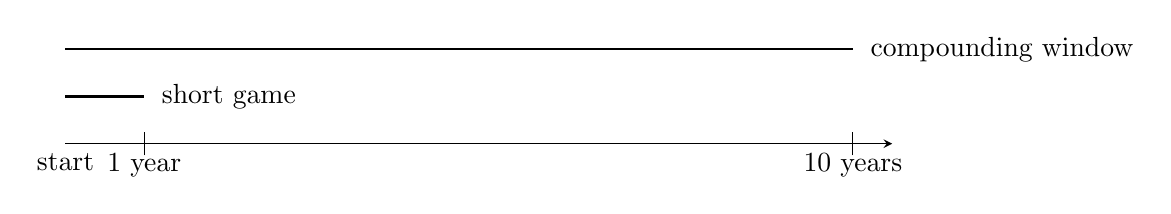
\begin{tikzpicture}[>=stealth]
\draw[->] (0,0) -- (10.5,0);
\draw (1,-0.15) -- (1,0.15);
\draw (10,-0.15) -- (10,0.15);
\draw[thick] (0,0.6) -- (1,0.6);
\draw[thick] (0,1.2) -- (10,1.2);

\node[below] at (0,0) {start};
\node[below] at (1,0) {1 year};
\node[below] at (10,0) {10 years};
\node[right] at (1.1,0.6) {short game};
\node[right] at (10.1,1.2) {compounding window};
\end{tikzpicture}
\end{figure}

At number \(10\), the lecture moves from time horizon to surface coverage. Mohammed Bingati says that the art of scale is the art of sales and marketing, and then gives the specific word the host wants to keep: omnipresence. One wants to be everywhere, at every time, and known by everyone. The clip's scale marker is again large:
\begin{equation}
Y_{\mathrm{Bingati}} \approx \$5{,}000{,}000{,}000.
\end{equation}

The host translates the doctrine into platform arithmetic. He says he has about three million followers on Facebook and makes more money there than on platforms where he has larger audiences:
\begin{equation}
F_{\mathrm{Facebook}} \approx 3 \times 10^6.
\end{equation}
That example matters because it prevents us from confusing presence with vanity. The relevant measure is not raw audience count; it is useful commercial coverage. A compact reconstruction is
\begin{equation}
P = \sum_i p_i,
\end{equation}
where \(p_i\) measures effective presence on channel \(i\).

The Hoffman lesson widens the clock. The Bingati lesson widens the map. The lecture wants both.

\section{Comfort, intelligence, and money while sleeping}

At number \(9\), the lecture turns from structure to disposition. The entrepreneur who sold BodyArmor to Coca-Cola for \(\$8\) billion is asked why, after exits of that scale, he is not content. The answer is sharp: one may be happy without being content. The host translates this into the lecture's preferred entrepreneurial moral. Comfort is not neutral. Comfort is a drift toward competitive softness.

At number \(8\), John Morgan, billionaire lawyer, attacks the mythology of solitary intelligence. The transcript is garbled around the cited Rockefeller book title, so the chapter must not lean on the title itself. The stable line is the one Morgan remembers and the host keeps: ``I hire scientists.'' One need not be the expert in every technical field. One must know how to locate expertise and put it to work.

\subsection{Question \& Answer}

Does one need to be the smartest person in the room? The lecture answers no. What is required is something more operational: one must be smart enough to know what kind of intelligence is missing, and disciplined enough to hire it. The founder's function here is not omniscience. It is selection, placement, and coordination.

At number \(7\), Joshua Crisp pushes the same reorientation into cash flow. He reports a year above \(\$11\) million and gives the lecture's familiar line: if one does not find a way to make money while sleeping, one will work until death. The host ties this line back to the Ashley Fox section. The richest people do not merely save. They invest, deploy, and build structures that continue paying when the founder is no longer in motion.

We should not over-formalize this part. The lecture does not. What it offers is a direction of travel: from labor-bound income toward capital-bound, system-bound, or distribution-bound income. The point is not to deny work at the beginning. It is to refuse a permanent dependence on direct exertion.

\section{Change, marketing, speed, and the size of the game}

At number \(6\), Jim Keyes gives the lecture's most explicit operator identity:
\begin{equation}
\text{Change} = \text{Opportunity}.
\end{equation}
If we leave it there, it sounds like a slogan. But Keyes does more than sloganize. He explains that if one responds to change while others resist it, the response becomes value. The useful reconstruction is therefore
\begin{equation}
\Delta E \longrightarrow A \longrightarrow V_{\mathrm{shareholder}},
\end{equation}
where \(\Delta E\) is a change in the environment, \(A\) the adaptive response, and \(V_{\mathrm{shareholder}}\) the value created by adapting better than competitors.

\begin{figure}[h]
\centering
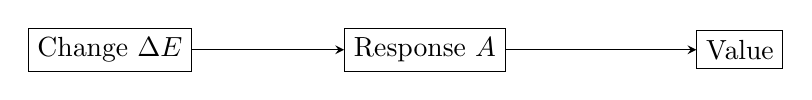
\begin{tikzpicture}[>=stealth]
\node[draw, rectangle] (change) at (0,0) {Change \(\Delta E\)};
\node[draw, rectangle] (adapt) at (4,0) {Response \(A\)};
\node[draw, rectangle] (value) at (8,0) {Value};

\draw[->] (change) -- (adapt);
\draw[->] (adapt) -- (value);
\end{tikzpicture}
\end{figure}

At number \(5\), Todd Johnson supplies the matching lesson on visibility. The clip is numerically anchored: roughly \(\$90\) to \(\$100\) million in company revenue in a year, and about \(\$25\) million for himself. The conclusion is that many people need what one offers; they simply do not know who one is. Marketing is therefore not cosmetic. It is the mechanism by which hidden value becomes purchasable value.

At number \(4\), the lecture accelerates. The Miami operator makes readiness identical with action. Procrastination is treated not as prudence but as failed commitment. The host condenses the lesson into the line he wants the audience to remember: start now.

Then comes number \(3\), and with it the lecture's most provocative heuristic.

\subsection{Question \& Answer}

Is a bigger game actually harder? The lecture says not in the simple way beginners assume. The speaker gives an escalating money ladder:
\begin{equation}
\$10^3,\ \ \$10^4,\ \ \$10^5,\ \ \$10^6,\ \ \$10^7,\ \ \$10^8.
\end{equation}
The host's gloss is twofold. First, very small clients often impose intense, penny-pinching pressure, while larger clients may have more capital and less fragility. Second, the lower end of the market is crowded because almost everyone is trained to think there. A cautious formalization is
\begin{equation}
m_1 < m_2 \Rightarrow c(m_1) > c(m_2),
\end{equation}
where \(m\) denotes the size of the problem being pursued and \(c(m)\) the density of competition around it.

This is not a law. It is a field heuristic. But it preserves the lecture's structure exactly. Bigger targets may not only pay more; they may also be less crowded.

\begin{figure}[h]
\centering
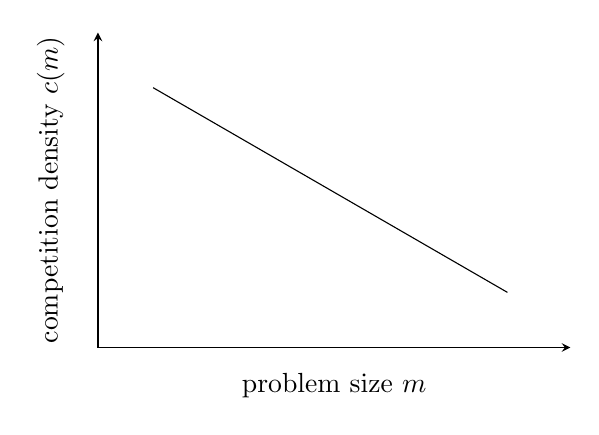
\begin{tikzpicture}[>=stealth]
\draw[->] (0,0) -- (6,0);
\draw[->] (0,0) -- (0,4);
\draw (0.7,3.3) -- (5.2,0.7);
\node[below] at (3,-0.2) {problem size \(m\)};
\node[rotate=90] at (-0.6,2) {competition density \(c(m)\)};
\end{tikzpicture}
\end{figure}

\section{Wings, ribbon, and the finite interval}

At number \(2\), Billy Ray Taylor turns the lecture away from business tactics toward self-trust. If a bird lands on a branch, does the bird trust the branch, or does it trust its wings? The host gives the correct reading: the branch is external support, but the wings are internal capability. The branch may fail. The wings are what keep the bird from dying with it.

A light symbolic rendering is
\begin{equation}
\mathrm{trust}(\mathrm{branch}) \neq \mathrm{trust}(\mathrm{wings}).
\end{equation}
This is not literal notation from the speaker. It is the gentlest way to keep the logical contrast visible. The entrepreneurial implication is plain: confidence cannot rest entirely on favorable conditions.

The lecture then prepares its final turn. The host says, in effect, that for number \(1\) he has no words of his own and will let Billy Ray Taylor explain. That surrender of commentary is important. The lecture deliberately lowers the host's voice right before the strongest demonstration.

At number \(1\), Taylor asks for a strip from \(1\) to \(100\). He marks the average female lifespan at about \(81\), the average male lifespan at about \(75\), and his own age at \(57\). Then he tears the ribbon in thought. The past is gone. The far tail may exist only in diminished quality. The remaining segment is what is actually available for use.

\subsection{Question \& Answer}

What exactly is left? In the roughest first pass, if \(a\) is current age and \(L\) is a reference lifespan, then
\begin{equation}
L_{\mathrm{rem}} = L - a.
\end{equation}
Using the speaker's own demonstration values,
\begin{align}
a &= 57, \\
L_{\mathrm{male}} &\approx 75, \\
L_{\mathrm{female}} &\approx 81,
\end{align}
and therefore
\begin{align}
L_{\mathrm{rem}}^{(75)} &\approx 18, \\
L_{\mathrm{rem}}^{(81)} &\approx 24.
\end{align}

But the lecture immediately refuses to let us stop at those two numbers. The late years do not necessarily have the same mobility, energy, or optionality as earlier years. So the true point is not demographic precision. It is finite interval arithmetic under quality loss. What has already been torn away cannot be recovered. What remains cannot be assumed equal in texture to what came before.

\begin{figure}[h]
\centering
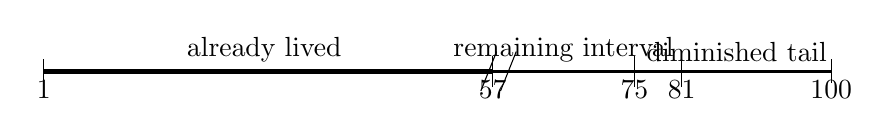
\begin{tikzpicture}[x=1cm,y=1cm]
\draw[line width=1pt] (0,0) -- (10,0);
\draw[line width=2pt] (0,0) -- (5.7,0);
\draw[dashed] (7.5,0) -- (10,0);

\draw (0,-0.15) -- (0,0.15);
\draw (5.7,-0.2) -- (5.7,0.2);
\draw (7.5,-0.2) -- (7.5,0.2);
\draw (8.1,-0.2) -- (8.1,0.2);
\draw (10,-0.15) -- (10,0.15);

\draw (5.55,-0.25) -- (5.75,0.25);
\draw (5.8,-0.25) -- (6.0,0.25);

\node[below] at (0,0) {1};
\node[below] at (5.7,0) {57};
\node[below] at (7.5,0) {75};
\node[below] at (8.1,0) {81};
\node[below] at (10,0) {100};

\node[above] at (2.8,0) {already lived};
\node[above] at (6.6,0) {remaining interval};
\node[above] at (8.8,0) {diminished tail};
\end{tikzpicture}
\end{figure}

That is why the lecture ends here rather than on net worth, exits, or marketing. The host explicitly says that this one conversation changed his perspective more than any other piece of business advice. The countdown resolves into mortality arithmetic. Tomorrow is not guaranteed, and the interval we still control is shorter than the mind pretends.

\section{Summary}

The lecture earns its seriousness by moving from spectacle into structure. It opens with montage, but the montage is only there to justify the reversal. Once the host becomes the object of inquiry, the numbers begin to matter: more than thirty billionaires interviewed, more than a thousand interviews overall, more than seven hundred thousand dollars in a recent month, more than six million on the year, and a business built from stacked revenue streams rather than a single line of income.

From there the countdown proceeds in order. First it filters advice. Then it explains how credibility precedes access. Then it shifts from saving to investing, from spending to retention, from a one-year frame to a ten-year frame, and from single-channel visibility to omnipresence. After that come the temperament lessons: do not get comfortable, hire intelligence, build income that can continue while you sleep, treat change as opportunity, make value visible through marketing, act before perfect conditions arrive, and do not assume that the small game is the easy game. Finally, the lecture closes where all of those tactics are judged: on self-trust and on the finite strip of time still available.

The mathematics remains modest, as it should. But it is real. The chapter turns on revenue decomposition, wealth update rules, retained capital, compounding horizon, channel coverage, adaptive response, competition density, and remaining interval. Those are enough to make the lecture coherent on the page, and enough to let the reader feel the countdown tightening step by step toward its last subtraction.